\section{Conversion: protocols and additional measurements}
\label{app:collective}\label{app:collective-data}
This appendix gives the experimental details behind \cref{sec:local}. We first describe the model pairs and the fixed prefixes used for measurement. We then ask where the teachers place their strongest requests, how well those requests produce parameter updates, and how the student's responsiveness changes during training. The derivations are in \cref{app:collective-proof,app:collective-frozen}.

\subsection{Setup}
\label{app:collective-protocol}
We compare two teachers for the same starting student at each scale. At 1.5B, the student is DeepSeek-R1-Distill-Qwen-1.5B and the teachers are JustRL-1.5B and DeepSeek-R1-Distill-Qwen-7B. At 7B, the student is DeepSeek-R1-Distill-Qwen-7B and the teachers are AceReason-Nemotron-7B and DeepSeek-R1-Distill-Qwen-14B. The AIME comparison uses 30 AIME 2024 problems at temperature $.6$. We draw 16 responses per problem at 1.5B and 4 at 7B.

At each scale, eleven rollouts from the initial student provide the prefixes for measurement. Each local kernel is computed from logit gradients with respect to all student parameters. Please note that, computing the gradients is expensive, the eigendecomposition itself is inexpensive. The kernel measurements therefore use sampled positions, while $\Xi$ serves as a less expensive monitor.


\subsection{Where the strongest requests occur}
\label{app:collective-types}
We analyze which kinds of positions receive the strongest teacher requests. The annotated rollouts contain 36,416 positions at 1.5B and 38,168 at 7B. For each teacher, the strongest $1\%$ contains 364 and 381 positions, respectively. 

\paragraph{Annotations and enrichment.}\label{app:semantic-protocol}
We use Opus 5 to label the sentences in the rollouts. Each sentence receives a semantic category, which describes its role in the reasoning. We also classify positions by their location within a sentence and by token kind. These are three separate classifications of the same positions, examined from different semantic aspects. We use the following prompt to create the semantic labels (this rubric is the result of iterating on the model's reasoning traces a few times, to settle on the most prevalent reasoning categories the model writes in its chain of thought).

\begin{promptbox}{LLM Judge Prompt}
\begin{Verbatim}[
    breaklines=true,
    breakanywhere=true,
    fontsize=\small,
    breaksymbolleft={}
]
You are annotating every sentence of a model's reasoning trace (for example, a model solving a math problem) with a label describing the act the sentence performs.

REASONING TRACE: "{reasoning_trace}"

Emit per sentence: {"sent_idx": int, "fine": [1 label], "uncertain": bool, "note": "..."} Read the FULL trace first; judge each sentence's FUNCTION IN CONTEXT.

## Fine labels

CONTROL family (steering the reasoning process):
- check-initiate: starting a verification act on ALREADY-ESTABLISHED material -- re-computing a prior result, re-reading the problem statement, re-deriving an earlier step. First-time testing of a fresh candidate or case is NOT check-initiate (see TECHNICAL).
- check-conclude: verdict closing a check episode. Covers: work-correctness verdicts ("Yes, that's correct", "that step was wrong"); verdicts about the check itself, including redundancy ("I already did this case", "we've already considered that"); resolutions of a problem re-read that settle interpretation ("So it's allowed to be prime").
- doubt-flag: hesitation OR bare deliberation cue WITHOUT an act ("Wait.", "Hmm, that seems too big.", "Let me think.", "Let's see."). Judged sentence-locally: a bare cue stays doubt-flag even when a check follows in the next sentence. Never label bare cues as plan.
- plan: stating an approach or opening a new sub-task, with the approach/task STATED ("I'll use coordinates", new-sub-task colon lead-ins like "Compute the exponent:"). Includes proceed-decisions ("Let me try that").
- reframe: abandoning/switching approach. NOT routine next-case moves in an enumeration ("Alternatively, x=2" = TECHNICAL).
- repair: announcing/making a correction of an earlier error.
- recap: MULTI-ITEM consolidation of established state used to steer. Single value-echoes = compute/derive.
- commit: FINAL-ANSWER commitment only ("So the answer is 34", "Answer: 34").

TECHNICAL family (object-level mathematics):
- derive: algebraic/logical derivation steps; this includes stating the associated problem facts, notation, coordinates, case setup, and within-computation connective lead-ins (including "Simplify:", "Comparing coefficients:").
- recall: invoking a theorem/definition/known mathematical fact.

OTHER family:
- style: pure filler/transition with no content and no steering.
- format: formatting artifacts, the end-of-reasoning marker (e.g. </think>), bare list numerals or LaTeX delimiters split onto their own lines (format, not fragment).
- unclear: genuinely unclassifiable.


## Fixed vocabulary and note rules
Use only the labels above; do not propose or introduce new labels. A sentence the rules do not settle or hard to classify takes the best available existing label, "uncertain": true, and leave a short note -- residual uncertainty is data itself, please do not treat it as a defect to legislate away. Furthermore, write in the note for the sentence if it genuinely has more than one of the labels above.
\end{Verbatim}
\end{promptbox}

%We compare the single-label semantic counts with counts that allow multiple labels; every headline enrichment value changes only by at most $0.1$.

For a category $c$, \emph{enrichment} compares its frequency among the teacher's strongest requests with its frequency among all annotated positions:
\[
 E_q(c)=\frac{\Pr(c\mid\text{strongest }1\%\text{ under teacher }q)}{\Pr(c)}.
\]

A value above 1 means that the category is more common among the strongest requests. For planning, we split the sentences in this class by position: their first three tokens (the opening of a plan) belong to the control family, and the remaining tokens (the stated approach) belong to the technical family; mixed sentences belong to neither. Panel~(a) of \cref{fig:conversion-tokens} takes each teacher's top 50\%, 20\%, 10\%, 5\%, 2\% and 1\% of requests and shows the share of sentence openings (first three tokens), control positions and technical positions, \emph{minus} the corresponding share among all annotated positions. \cref{fig:request-trends} shows the raw shares. Bootstrap intervals resample the annotated rollouts. They are computed separately for each teacher. Panels~(b, c) of \cref{fig:conversion-tokens} show twelve selected rows, and \cref{fig:composition} shows the full set. \Cref{tab:semantic-enrichment} gives the values used in the main figure.

\paragraph{Differences between teachers.}
At 1.5B, planning openings are enriched $3.59\times$ under the sibling teacher and $0.30\times$ under the larger teacher. Sentence-initial positions are enriched $2.91\times$ and $1.46\times$, respectively. At 7B, the sibling teacher places relatively more of its strongest requests at reframing, checking, and doubt positions. Wait-family tokens are enriched $4.50\times$ under the sibling and $1.23\times$ under the larger teacher.

The difference depends on the category.  At 7B, planning openings are enriched $4.13\times$ and $1.06\times$, while the stated approach of a plan is enriched $0.72\times$ and $1.70\times$; the teachers' derivation enrichment is similar ($0.84\times$ and $0.83\times$). Digit-bearing positions are relatively more prominent under the larger teacher at both scales.

We find that, as the percentile goes up, the sibling teacher's shares of \emph{sentence openings and control positions} grow relative to all positions, while the larger teacher's return to or fall below them (\cref{fig:request-trends}). Among the strongest 1\%, the sibling teacher's share of sentence openings exceeds the larger teacher's by $19.2$ [$13.1$, $27.7$] percentage points at 1.5B and $27.6$ [$18.8$, $37.0$] at 7B.

\begin{figure}[ht]
\centering
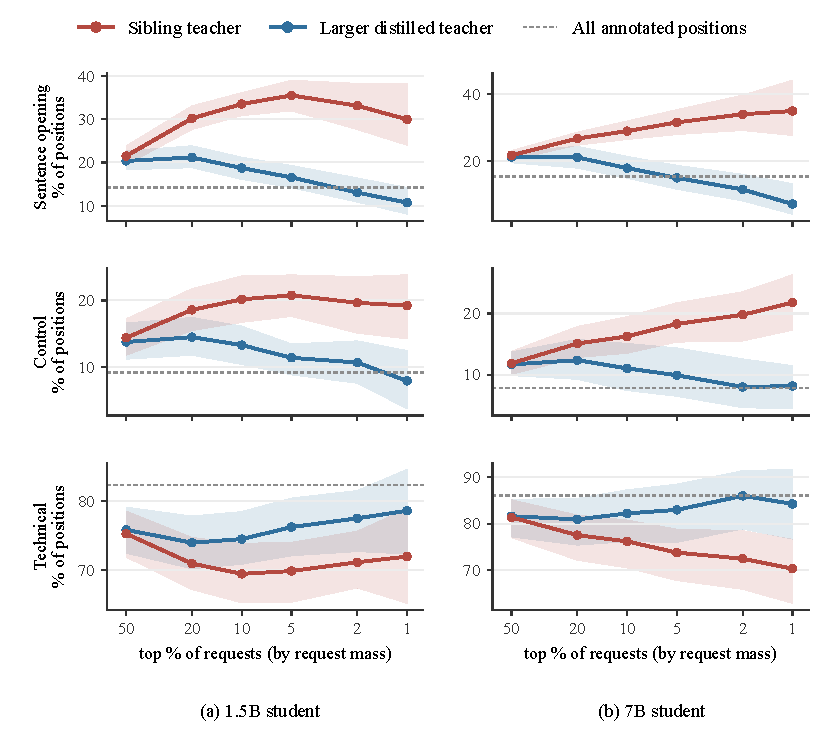
\includegraphics[width=\linewidth]{figures/section42/fig_request_trends_by_scale.pdf}
\caption{\textbf{Composition of the strongest requests as the percentile rises.} Shares of sentence openings (first three tokens), control positions and technical positions among each teacher's top 50\%, 20\%, \ldots, 1\% of requests. Dotted: all annotated positions; bands: 95\% bootstrap intervals over the annotated rollouts.}
\label{fig:request-trends}
\end{figure}

\begin{table}[ht]
\centering\small
\begin{tabular}{lrrrr}
\toprule
& \multicolumn{2}{c}{1.5B student} & \multicolumn{2}{c}{7B student} \\
\cmidrule(lr){2-3}\cmidrule(lr){4-5}
Position category & Sibling & Larger & Sibling & Larger \\
\midrule
Reframe & 1.63 & 0.70 & 2.61 & 0.65 \\
Check-conclude & 1.52 & 0.91 & 1.86 & 0.62 \\
Doubt flag & 1.15 & 1.84 & 2.95 & 0.68 \\
Check-initiate & 1.37 & 1.20 & 2.64 & 1.32 \\
Planning: opening & 3.59 & 0.30 & 4.13 & 1.06 \\
Recap & 1.48 & 1.11 & 0.00 & 2.31 \\
Planning: stated approach & 1.62 & 0.96 & 0.72 & 1.70 \\
Derivation & 0.78 & 0.93 & 0.84 & 0.83 \\
Recall & 2.04 & 1.89 & 0.50 & 2.18 \\
Mixed & 0.98 & 1.57 & 1.25 & 1.25 \\
\midrule
Wait-family token & 1.74 & 0.43 & 4.50 & 1.23 \\
Digit-bearing token & 0.65 & 0.85 & 0.40 & 0.79 \\
\bottomrule
\end{tabular}
\caption{\textbf{Enrichment values for the main semantic figure.} Each value compares the frequency of a category among the strongest requests with its frequency among all annotated positions. \Cref{fig:composition} shows the bootstrap intervals for each teacher.}
\label{tab:semantic-enrichment}
\end{table}

\begin{figure}[ht]
\centering
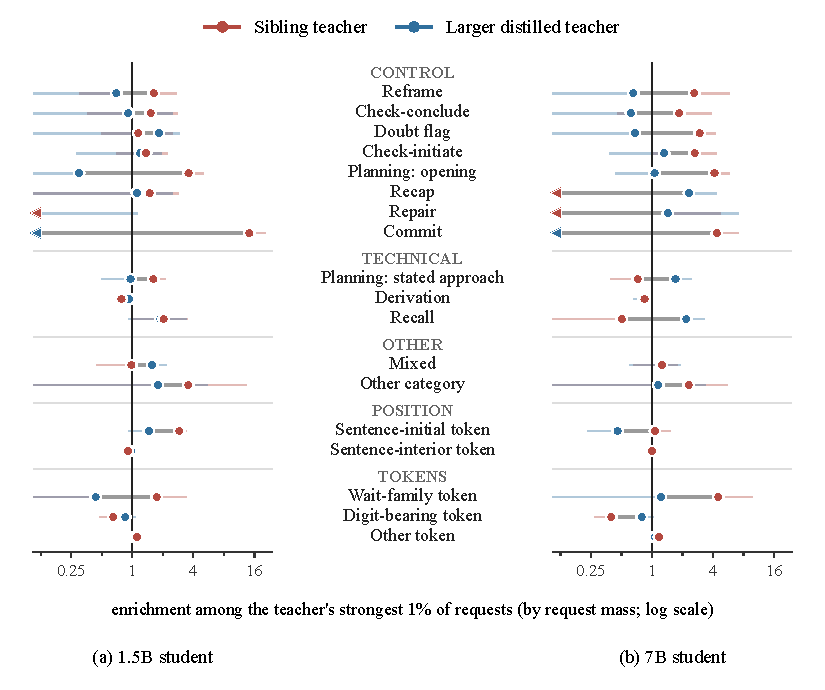
\includegraphics[width=\linewidth]{figures/section42/fig_request_fields_full.pdf}
\caption{\textbf{Where the strongest requests occur.} The full set of semantic categories, sentence positions, and token kinds. A ratio of one means that a category has the same frequency among the strongest requests as in the annotated rollouts. Planning sentences are split into their opening and stated approach. Intervals are clipped at the plot edges; left-pointing markers denote estimates below the plotted range, including zero. The main figure selects twelve rows.}
\label{fig:composition}
\end{figure}

\FloatBarrier
\Needspace{10\baselineskip}
\subsection{Conversion estimates by semantic class}
\label{app:collective-conventions}
We now ask which factors in \cref{eq:pac} distinguish the healthy and stalled runs. We report pressure $P$, accessibility $A$, and coherence $C$ separately for the \textsc{control} and \textsc{technical} samples selected for each teacher. The initial comparison asks how the same starting student responds to the two teachers. The endpoint comparison asks how much disagreement remains and how the student's responsiveness has changed.

\paragraph{Measurement and estimation.}
We save the training rollouts and the request vector $B$ computed at every position during training. The initial requests $B_0$ used in the frozen-request probes come directly from these records. For a fixed request at prefix $s$, the parameter gradient is $g_t(s)=\Phi_t(s)^\top B(s)$. We obtain it by backpropagating through $B(s)^\top z_t(s)$ while holding $B(s)$ constant.

The squared norm of a sample mean includes sampling variance. We correct for this before estimating coherence. For $n>1$ sampled gradients, write $\bar g=n^{-1}\sum_i g_i$ and $\widehat D_g=n^{-1}\sum_i\|g_i\|^2$. The correction is
\[
 \widehat C_{\mathrm{corr}}=
 \frac{\left(\|\bar g\|^2-
       [\widehat D_g-\|\bar g\|^2]/(n-1)\right)_+}{\widehat D_g},
 \qquad \widehat D_g>0,
\]
where $(r)_+=\max(r,0)$. Under independent sampling, the numerator before truncation is unbiased for the squared norm of the population-mean gradient (\cref{prop:gradient-norm-correction}). 

\begin{table}[htb]
\centering\small\setlength{\tabcolsep}{4.2pt}
\begin{tabular}{llrrrrr}
\toprule
Run & Class & $P_0$ & $A_0/10^3$ & $C_0$ & $\Xi_0/10^3$ & $\|u_0\|$ \\
\midrule
7B healthy & Control & 0.192 & 119.8 & 0.081 & 9.70 & 43.1 \\
7B healthy & Technical & 0.151 & 106.3 & 0.055 & 5.85 & 29.7 \\
7B stalled & Control & 0.521 & 148.1 & 0.025 & 3.70 & 43.9 \\
7B stalled & Technical & 0.599 & 128.8 & 0.020 & 2.58 & 39.3 \\
1.5B healthy & Control & 6.024 & 39.6 & 0.041 & 1.62 & 98.9 \\
1.5B healthy & Technical & 2.569 & 54.5 & 0.064 & 3.49 & 94.7 \\
1.5B stalled & Control & 0.824 & 41.3 & 0.040 & 1.65 & 36.9 \\
1.5B stalled & Technical & 1.110 & 53.8 & 0.039 & 2.10 & 48.2 \\
\bottomrule
\end{tabular}

\caption{\textbf{Initial conversion estimates by semantic class.} Each row uses $n=80$ positions selected for one teacher and class. $P$ and $A$ use measurements at individual positions. $C$ uses the finite-sample correction above. $\Xi$ and $\|u\|$ are approximate values computed from these estimates. Comparisons are within scale and parameterization.}
\label{tab:collective-initial}
\end{table}

\paragraph{Initial comparison.}
\Cref{tab:collective-initial} shows why gradient norm alone does not explain conversion. At 7B, the healthy run has somewhat lower accessibility but $2.75$--$3.24\times$ higher coherence across the two classes. Its collective gain is $2.27$--$2.62\times$ higher. The stalled run still has a comparable or larger gradient norm because its request pressure is higher.

At 1.5B, accessibility is similar between the two teachers, and the coherence difference depends on the class. The initial collective gains are nearly equal in \textsc{control}: $1.62$ versus $1.65$, in units of $10^3$. In \textsc{technical}, the healthy run has the larger gain: $3.49$ versus $2.10$. Thus its larger gradient norms do not imply a larger conversion gain in every class.

\paragraph{Remaining requests and responsiveness.}
\Cref{tab:collective-endpoints} separates two endpoint comparisons. The live conversion factors use the current requests $B_t$. They measure the response to the remaining disagreements with the teacher. The last column instead reapplies the initial requests $B_0$. With both the requests and prefixes fixed, this column measures how local responsiveness to those requests has changed.

\begin{table}[htb]
\centering\footnotesize\setlength{\tabcolsep}{3.2pt}
\begin{tabular}{llrrrrrr}
\toprule
Run & Class & Step & $P_t/P_0$ & $A_t/A_0$ & $C_t/C_0$ & $\Xi_t/\Xi_0$ & $A_t[B_0]/A_0[B_0]$ \\
\midrule
7B healthy & Control & 200 & 0.005 & 0.983 & 0.012 & 0.012 & 1.414 \\
7B healthy & Technical & 200 & 0.007 & 2.159 & 0.036 & 0.079 & 1.232 \\
7B stalled & Control & 150 & 0.740 & 0.827 & 0.520 & 0.430 & 0.810 \\
7B stalled & Technical & 150 & 0.740 & 0.884 & 0.500 & 0.442 & 0.889 \\
1.5B healthy & Control & 200 & 0.009 & 1.216 & 0.341 & 0.415 & 2.829 \\
1.5B healthy & Technical & 200 & 0.015 & 3.628 & 0.031 & 0.113 & 5.399 \\
1.5B stalled & Control & 200 & 0.602 & 0.836 & 0.725 & 0.606 & 0.831 \\
1.5B stalled & Technical & 200 & 0.790 & 0.793 & 0.564 & 0.447 & 0.789 \\
\bottomrule
\end{tabular}

\caption{\textbf{Remaining requests and responsiveness at the endpoint.} The positions are the same as at initialization. The pressure and live conversion columns use the current requests $B_t$; the last column uses the initial requests $B_0$. All diagnostic columns are ratios to their initial values. Endpoints are step 200, except for stalled 7B at step 150. Coherence estimates are rounded, especially at healthy endpoints.}
\label{tab:collective-endpoints}
\end{table}

The healthy runs retain only $0.5$--$1.5\%$ of their initial request energy. The stalled runs retain $60.2$--$79.0\%$. Meanwhile, accessibility to the initial requests increases in both classes of each healthy run and decreases in both classes of each stalled run.

\FloatBarrier
\Needspace{10\baselineskip}
\subsection{How the local kernel changes}
\label{app:collective-geometry}
To understand the change in responsiveness, we measure both the strength and movement of the kernel's leading directions. At each prefix $s$, let $V_{t,3}(s)$ contain the orthonormal eigenvectors of the symmetrized local kernel $K_t(s,s)$ with the three largest eigenvalues. Denote those eigenvalues by $\{\lambda_{j,t}(s)\}_{j=1}^3$. Main Figure~\ref{fig:conversion-geometry} plots
\[
 G_3(s,t)=\frac{\sum_{j=1}^3\lambda_{j,t}(s)}{\sum_{j=1}^3\lambda_{j,0}(s)},
 \qquad
 O_3(s,t)=\frac{\|V_{0,3}(s)^\top V_{t,3}(s)\|_F^2}{3}.
\]
$G_3$ measures the change in the sum of the three largest eigenvalues. $O_3$ measures how much their subspace overlaps with its initial position. It is the mean squared cosine of the three principal angles: $1$ means identical subspaces and $0$ means orthogonal subspaces. The main figure reports median $G_3$ and $O_3$ over 160 positions; the table below reports $1-O_3$ instead. Moreover, subspace movement alone does not tell us whether the kernel becomes better or worse aligned with the teacher's requests. For this, we measure the share of the initial request in the leading subspace, $w_{1:3}(s,t)=\sum_{j\leq3}|v_{j,t}^\top b_0|^2$, where $b_0$ is the unit direction of the initial request. Its change is $\Delta w_{1:3}$. \Cref{fig:conversion-turn} compares this change for the two teachers' requests in the same checkpoint kernel.

\begin{table}[htb]
\centering\small\setlength{\tabcolsep}{3.4pt}
\begin{tabular}{lrrrrrr}
\toprule
Run & Step & $G_3$ & $1-O_3$ & $\Delta w_{1:3}$ (pp) & Median $a_t/a_0$ & $A_t[B_0]/A_0[B_0]$ \\
\midrule
7B healthy & 50 & 1.19 & 0.034 & -0.23 & 1.04 & 1.23 \\
7B healthy & 200 & 1.25 & 0.041 & -0.36 & 1.07 & 1.34 \\
7B stalled & 50 & 0.79 & 0.018 & +1.12 & 0.93 & 0.90 \\
7B stalled & 150 & 0.74 & 0.032 & +1.51 & 0.91 & 0.85 \\
1.5B healthy & 50 & 1.00 & 0.232 & +5.49 & 1.19 & 3.95 \\
1.5B healthy & 200 & 2.31 & 0.369 & +5.07 & 2.08 & 3.78 \\
1.5B stalled & 50 & 0.80 & 0.022 & +1.06 & 0.91 & 0.86 \\
1.5B stalled & 200 & 0.67 & 0.044 & +0.89 & 0.83 & 0.80 \\
\bottomrule
\end{tabular}

\caption{\textbf{Changes in local geometry.} Except in the last column, ratios and differences are computed at each position before taking the median. The last column compares accessibility averaged across positions with weights proportional to initial request energy. The median and weighted average describe different aspects of the same sample. Here pp denotes percentage points.}
\label{tab:collective-geometry}
\end{table}

Early on in training (by step 50), the healthy 1.5B run has already changed its leading subspace, while the leading strength is near its initial value. The strength increases later. The healthy 7B run mainly increases leading strength, with little subspace movement. Both stalled runs lose leading strength.

The table also distinguishes a typical position from an average weighted by request energy. For example, at step 50 of healthy 1.5B, the median sensitivity ratio is $1.19$, while the ratio of weighted accessibilities is $3.95$. The latter gives more weight to positions with larger initial requests. Their difference reflects the weighting and the way results are combined across positions.

\begin{figure}[htb]
\centering
\begin{subfigure}[t]{.48\linewidth}
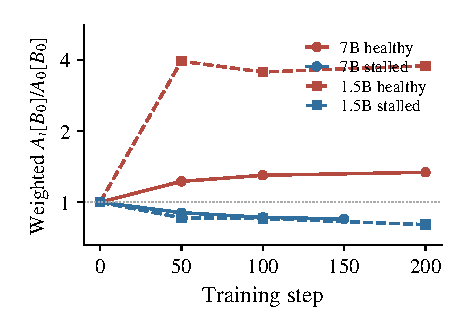
\includegraphics[width=\linewidth]{figures/section42/frozen_access.pdf}
\caption{Accessibility to the initial requests.}
\end{subfigure}\hfill
\begin{subfigure}[t]{.48\linewidth}
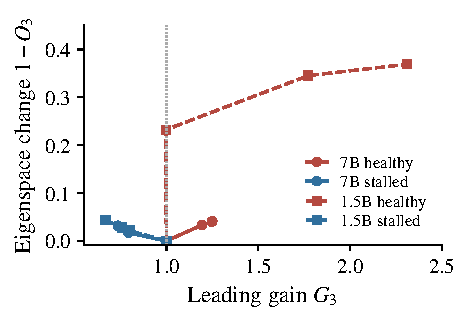
\includegraphics[width=\linewidth]{figures/section42/eigenframe.pdf}
\caption{Strength and movement of the leading subspace.}
\end{subfigure}
\caption{\textbf{Changes in the kernel and its response to the initial requests.} Left: $A_t[B_0]/A_0[B_0]$ on the combined sample, with equal numbers of positions from the two classes. Right: median leading strength and subspace change across positions. Red/blue denote healthy/stalled runs; circles/squares denote 7B/1.5B.}
\label{fig:collective-supplement}
\end{figure}

\Cref{fig:collective-spectra} extends the comparison to the full eigenvalue profile. It compares eigenvalues at the same sorted rank across checkpoints. It is clear that the healthy runs experience a lift in the principal eigenvalues as training proceeds, while the stalled runs experience a decline instead.

\begin{figure}[htb]
\centering
\begin{subfigure}[t]{.48\linewidth}
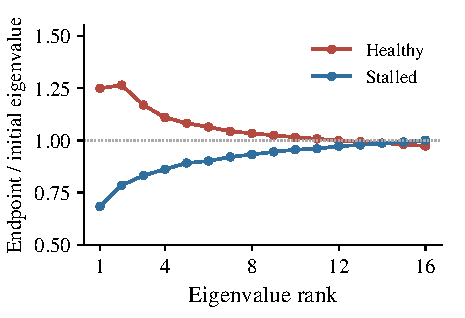
\includegraphics[width=\linewidth]{figures/section42/spectra_7B.pdf}
\caption{7B student.}
\end{subfigure}\hfill
\begin{subfigure}[t]{.48\linewidth}
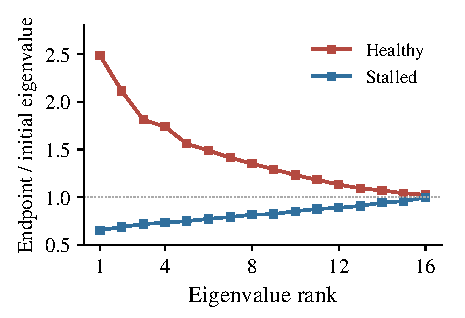
\includegraphics[width=\linewidth]{figures/section42/spectra_1p5B.pdf}
\caption{1.5B student.}
\end{subfigure}
\caption{\textbf{Endpoint eigenvalues relative to initialization.} At each sorted rank, we compute the endpoint-to-initial ratio at each position and report the median over 160 positions per run. Red/blue denote healthy/stalled runs. Endpoints are step 200, except for stalled 7B at step 150.}
\label{fig:collective-spectra}
\end{figure}

A separate comparison groups initial directions by their request energy. The reported growth is not concentrated in the groups with stronger requests. We therefore distinguish a turn toward the teacher's requests from preferential growth along the most strongly requested initial directions.


\FloatBarrier
\Needspace{10\baselineskip}
\subsection{Alignment with the teacher}
\label{app:collective-specificity}
The leading subspace rotates in the healthy 1.5B run. Does this movement favor the teacher that trained the student? We compare the training-run teacher's initial requests with the other teacher's initial requests at the same prefixes and token coordinates. Both are evaluated in the same checkpoint kernel. More precisely, at each position, we subtract their changes in projection onto the leading subspace:
\[
 d_s(t)=\Delta w_{1:3}^{\mathrm{trained}}(s,t)
       -\Delta w_{1:3}^{\mathrm{other}}(s,t).
\]
A positive value means that the training teacher's requests gain more projection. \Cref{fig:conversion-turn} uses step 50 for all four runs. The comparison holds the kernel change fixed and asks which field gains more projection.

\begin{table}[htb]
\centering\small\setlength{\tabcolsep}{3.5pt}
\begin{tabular}{lrrrr}
\toprule
Run & Trained gain (pp) & Other gain (pp) & Paired difference (pp) & 95\% interval \\
\midrule
7B healthy & -0.23 & +0.07 & -0.16 & $[-0.33,+0.27]$ \\
7B stalled & +1.12 & +1.25 & +0.00 & $[-0.53,+0.60]$ \\
1.5B healthy & +5.49 & +2.42 & +1.79 & $[+0.94,+3.13]$ \\
1.5B stalled & +1.06 & +1.00 & -0.16 & $[-0.29,+0.05]$ \\
\bottomrule
\end{tabular}

\caption{\textbf{Comparison of the two teachers' requests at step 50.} Values are medians over the same 160 positions. The paired difference is the median of the per-position differences. For each of 3,000 bootstrap samples, we resample the eleven initial rollouts and retain all selected positions in each sampled rollout. The two fields remain paired and the trained checkpoints remain fixed.}
\label{tab:collective-specificity}
\end{table}

The healthy 1.5B run has a median paired difference of $1.79$ percentage points, with a $95\%$ interval of $[0.94,3.13]$. The other three intervals include zero. These measurements show that there is a ``preferential'' turn toward the training teacher's requests in healthy 1.5B. The paired median need not equal the difference between the two separate medians: $5.49-2.42$ and $1.79$ summarize the same positions in different orders. The bootstrap measures variation across the sampled rollouts with the trained checkpoints fixed.

